% -*- coding: utf-8 -*-
\documentclass[11pt]{article}
\usepackage[UTF8]{ctex}
\usepackage{graphicx}
\usepackage[a4paper, body={18cm,22cm}]{geometry}
\usepackage{amsmath,amssymb,amstext,wasysym,enumerate,graphicx}
\usepackage{float,abstract,booktabs,indentfirst,amsmath}
\usepackage{array}
\usepackage{booktabs}
\usepackage{multirow}
\usepackage{diagbox}
\renewcommand\arraystretch{1.4}
\usepackage{indentfirst}
\usepackage{caption}
\usepackage[colorlinks,linkcolor=blue]{hyperref}
\usepackage{algorithm}
\usepackage{algorithmicx}
\usepackage{algpseudocode}
\setlength{\parindent}{2em}

\geometry{left=2.8cm,right=2.2cm,top=2.5cm,bottom=2.5cm}
%\geometry{left=3.18cm,right=3.18cm,top=2.54cm,bottom=2.54cm}

\title{\LARGE \bf Squarified Treemap算法作业报告}
\author{\LARGE 张启哲 \quad 1900011638}
\date{\Large \today}

\begin{document}
	\maketitle
	
	\vspace{40pt}
	
	\begin{figure}[h]
		\centering
		
\includegraphics[width=8cm]{./figures/pku.jpg}
	\end{figure}

	\vspace{40pt}
	
	\renewcommand{\contentsname}{目录(Contents)}
	\renewcommand{\algorithmicrequire}{\textbf{Input:}}
	\renewcommand{\algorithmicensure}{\textbf{Output:}}
	
	\tableofcontents
	
	\thispagestyle{empty}
	
	\newpage
	
	\setcounter{page}{1}
	
	\section{数据描述与分析(Data Description and Analysis)}
	\subsection{数据描述}
	本次可视化作业使用的数据是来自于\href{https://projects.iq.harvard.edu/cbdb/data-sets}{China Biographical Database Project(CBDB)}中Ming Jinshi List的明进士数据。数据集包括明代52年科举考试的所有进士原始资料,共14116人。
	
	\hspace*{\fill} \\
	
	数据集以excel数据xlsx的格式呈现,共有3个工作表。第1个工作表Ming Jinshi Lists中包括了所有进士的详细信息,第2个工作表Release Notes中描述了3个工作表中的内容并列出了各次科举考试的年份和资料出处,第3个工作表dazi rule描述了进士数据项的格式。
	
	\subsection{数据分析}
	本次可视化算法Squarified Treemap处理的是层次数据,根据首个工作表中的各项目属性,选择籍贯一项进行处理。明代的行政区划大致可分为司府州县4级与司州县、司府州3级两种制度并存,在本次作业中主要将籍贯按照级别划分为3类:司、府(州)、州(县),府与州合并,将直隶州与府视为同一级别处理,州与县合并,县归属于非直隶的州管理,无归属的则视为与州同一级别的独立行政单位。此外,明代还设有专门的军籍制度,下设卫、所,本次作业将卫所合并视为与司同一级的行政单位,而分别视为与府同一级的行政单位,以下不分(许多带有地域的卫所的治所并不在当地,因此将其划为当地也不妥)。
	
	\subsection{数据清洗}
	本次作业在清洗数据时首先将xlsx格式的数据转化为json格式的数据,之后根据各级行政单位逐级拆分,部分含有罕用字的籍贯再安装了Unicode extension A \& B后依然无法读取,这部分籍贯被划为未知(数量较少),同时有极少数特殊籍贯(如高丽等)也做了同样处理。
	
	\hspace*{\fill} \\
	
	值得一提的是,原始数据中的许多籍贯在录入时没有记录上一级行政单位,为了形成层次结构数据,处理时首先将数据集扫描一遍,记录其中已知的行政区划从属关系,在第二遍处理数据时便可以将大多数无上级行政单位的籍贯正确划分(例如第1位进士的籍贯是X府Y州,第2位的是Y州,此时原始数据未记录第2位进士所属的府,但可以通过第2位进士的籍贯将第2位正确划分为X府),剩余的小部分未知归属划为已知最低一级行政单位下的其他分支。
	
	\hspace*{\fill} \\
	
	另外,在较长的时间推移中,不少地名出现了演变,如宁波又名明州、宁江、顺天又名北平等,不少地名中出现异体字(即同一个字有不同的写法),如“凉”与“涼”、“寜”与“寍”等,还有原始数据在录入时可能存在错别字的现象,如将莱州误记为菜州、绍兴误记为照兴等,本次作业在清洗数据时均已充分考虑,并最大限度地保证清洗过后数据的真实性(具体细节在数据处理文件中可见)。同时,原始数据在南直隶与北直隶上未作区分,统一记为直隶,但考虑到南北直隶在实际地理位置上有较大差别,本次作业将这两个直隶司在数据清洗时进行了拆分。
	
\newpage
	\section{算法设计与分析(Algorithm Design and Analysis)}
	本次作业中的算法直接复现了Mark Bruls, Kees Huizing, and Jarke J. van Wijk的论文\href{http://vis.pku.edu.cn/course/visclass_f21/material/Squarified_Treemap.pdf}{Squarified Treemaps}中的算法(算法实现细节在js文件中可见)。
	
	其中主算法squarify通过递归的方式实现:
	
	\begin{algorithm}[h]
		\caption{squarify}
		\begin{algorithmic}[1]
			\Require
			children: list of child nodes;
			row: list of nodes in current row;
			w: width of current row.
			\If {children == []} 
			\If {row != []} \State layoutrow(row, w);
			\EndIf
			\State return;
			\EndIf
			\State var node = children[0];
			\If {worst(row, w) >= worst(row++[node], w)}
			\State squarify(row-\--[node], row++[node], w);
			\Else \State layoutrow(row, w);
			\State squarify(children, [], min(rwidth, rheight));
			\EndIf
		\end{algorithmic}
	\end{algorithm}

	其中[]代表空列表,++和-\--分别代表列表元素的增添和删除,layoutrow只是简单地记录已经确定并摆放好位置的一行矩形,worst则是计算一行矩形中的最大长宽比,实现如下:
	
	\begin{algorithm}[h]
		\caption{worst}
		\begin{algorithmic}[1]
			\Require
			row: list of nodes in current row;
			w: width of current row.
			\Ensure
			ratio: highest aspect ratio of current row.
			\State var s = sum(row);
			\State var $r^+$ = max(row);
			\State var $r^-$ = min(row);
			\State ratio = max($(w^2r^+)/(s^2), (s^2)/(w^2r^-)$);
		\end{algorithmic}
	\end{algorithm}
	
	而rwidth与rheight则是指剩余矩形的宽与高(这里省去了原算法中的width()函数)。
	
	\hspace*{\fill} \\
	
	注:在绘制树图时引入parent属性来分配颜色,一级子结点的parent设置为自己,其余子结点的parent都递归地设置为父结点,使得颜色按照第一级行政区划(司)分配;每个小矩形的颜色透明度与字号大小都与面积正相关,以使整个树图更加直观与美观。同时可视化实现中加入了用户交互,上方按钮条可以选择展示的行政区划级别,用户将鼠标放置在小矩形上时对应矩形会高亮显示,鼠标点击时会弹出该矩形对应的行政区划名称与进士总人数。
	
	\section{可视化结果描述(Visualization Result Description)}
	\subsection{结果展示}
	\begin{figure}[H]
		\centering
		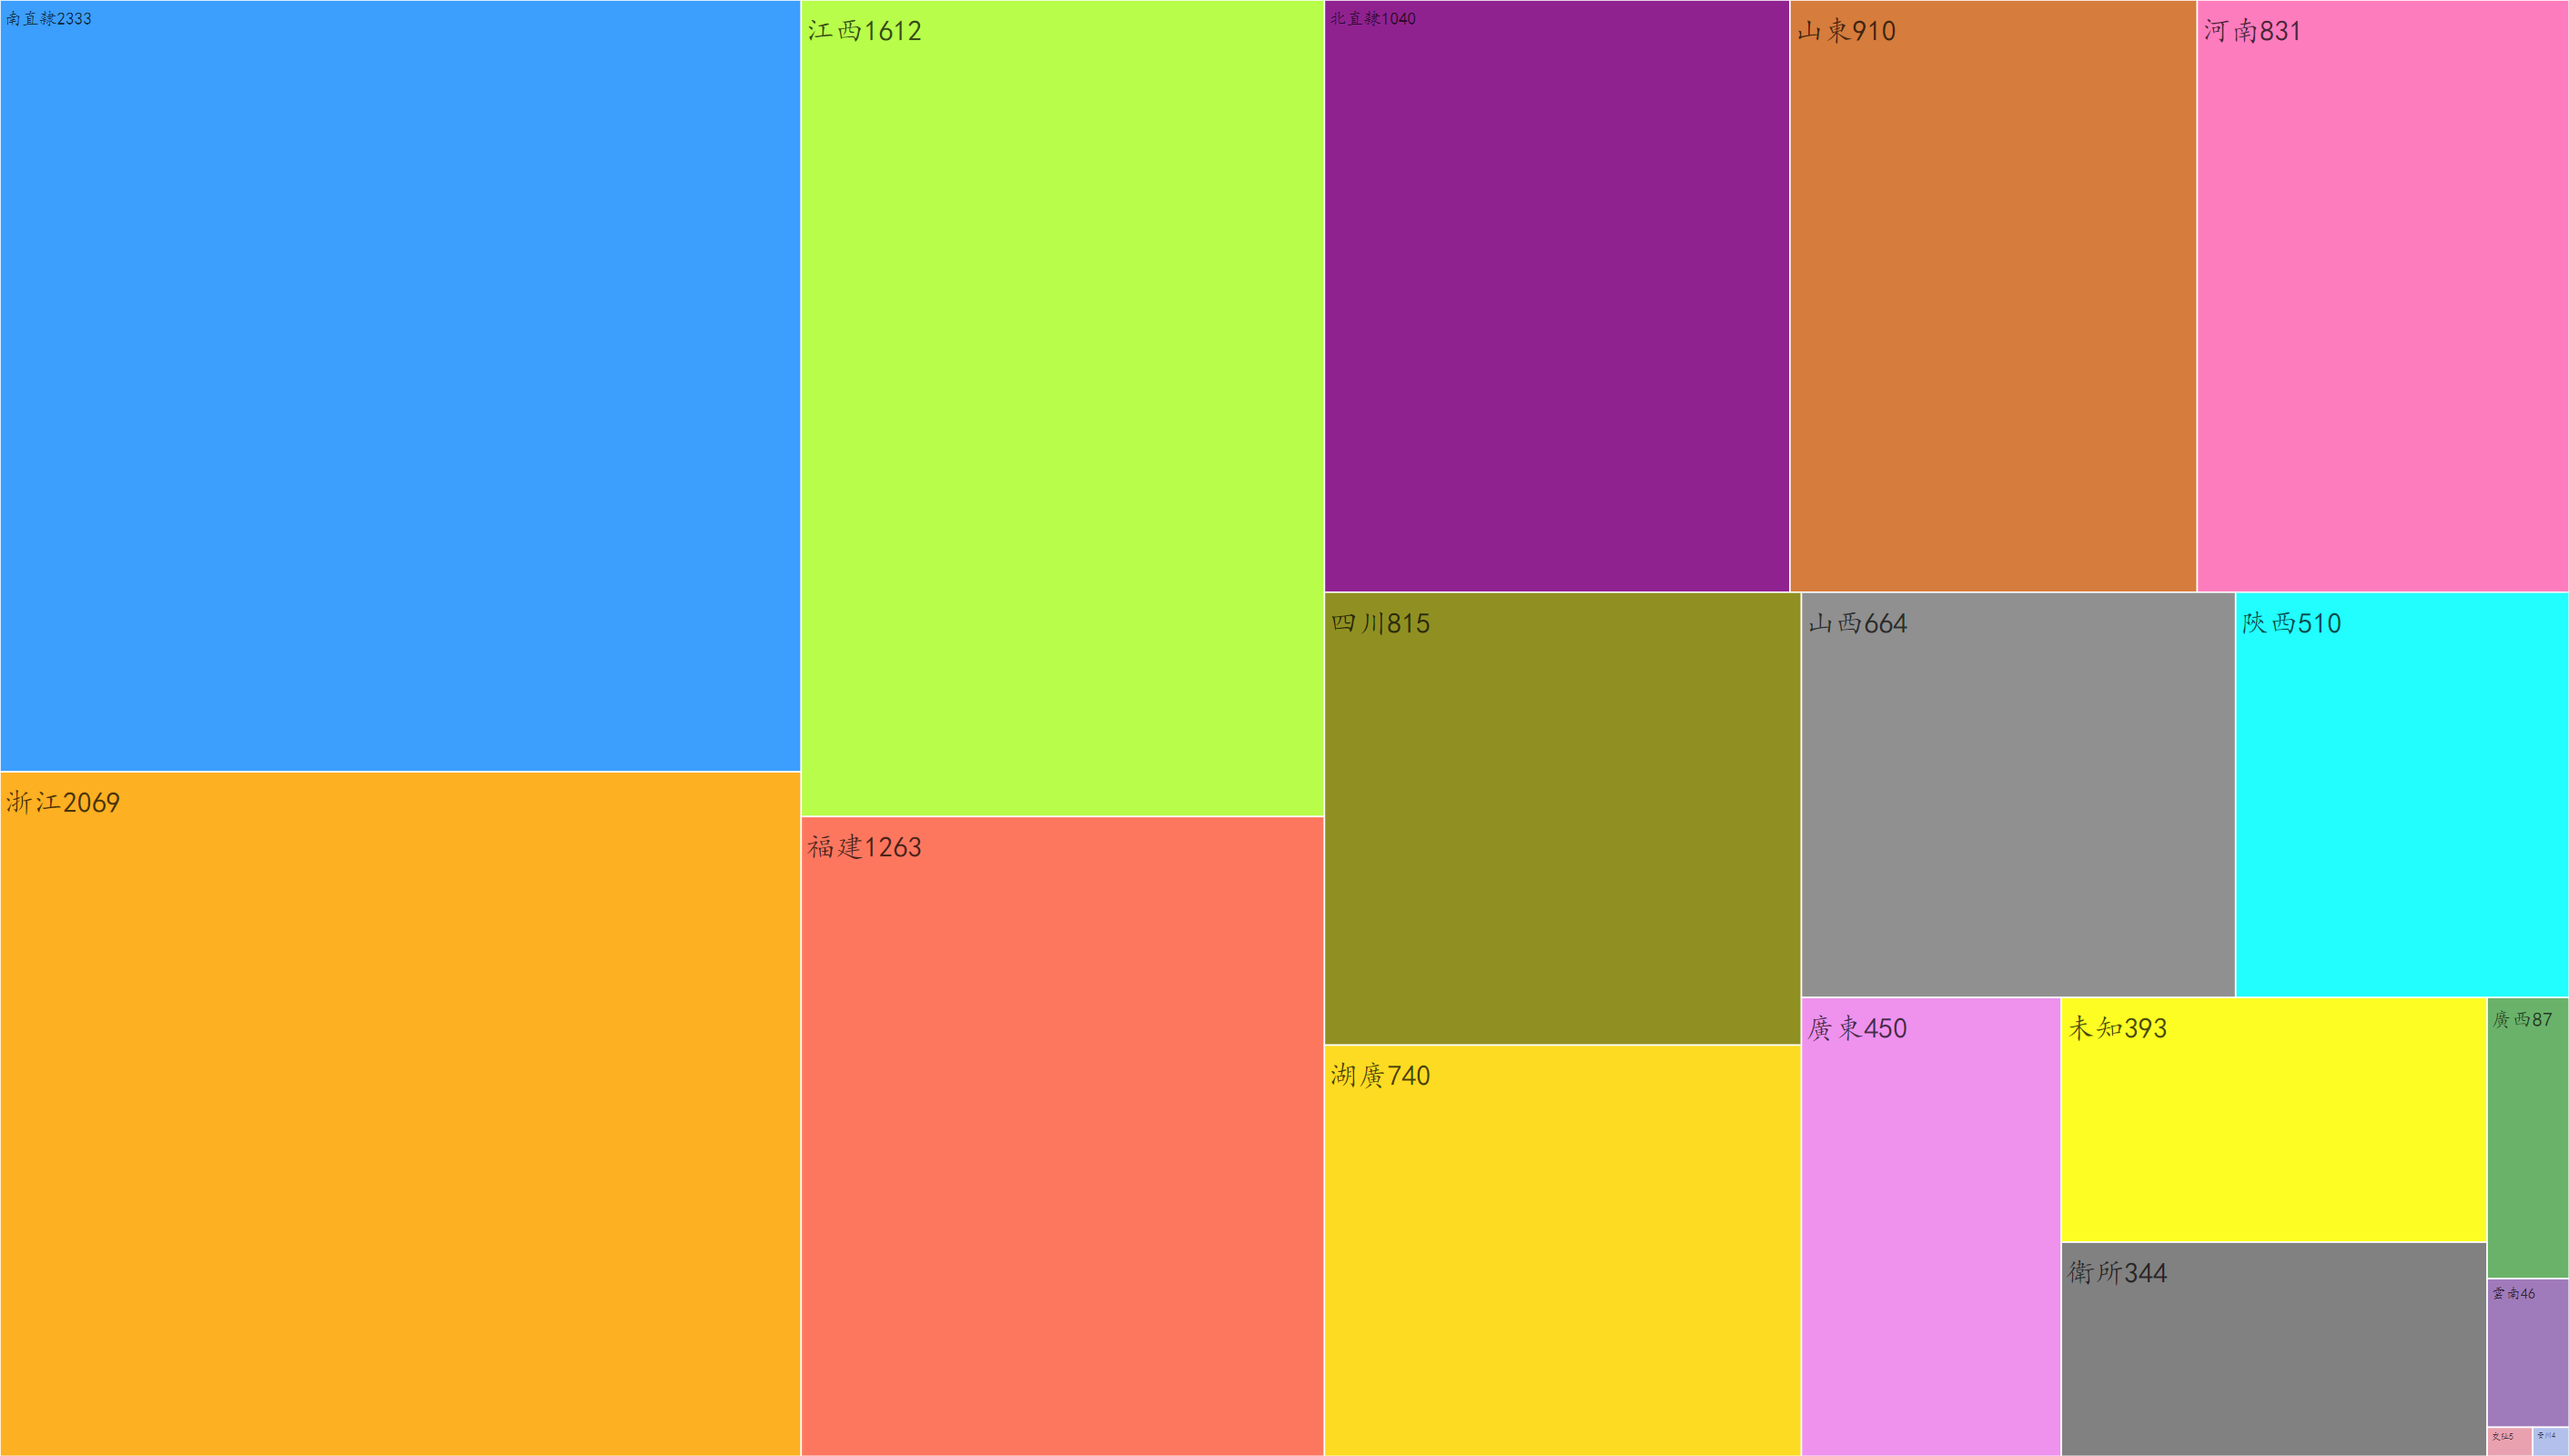
\includegraphics[width=10cm]{./figures/si_squarified_treemap.png}
		\caption{Squarified Treemap of Si-level}
	\end{figure}
	\begin{figure}[H]
		\centering
		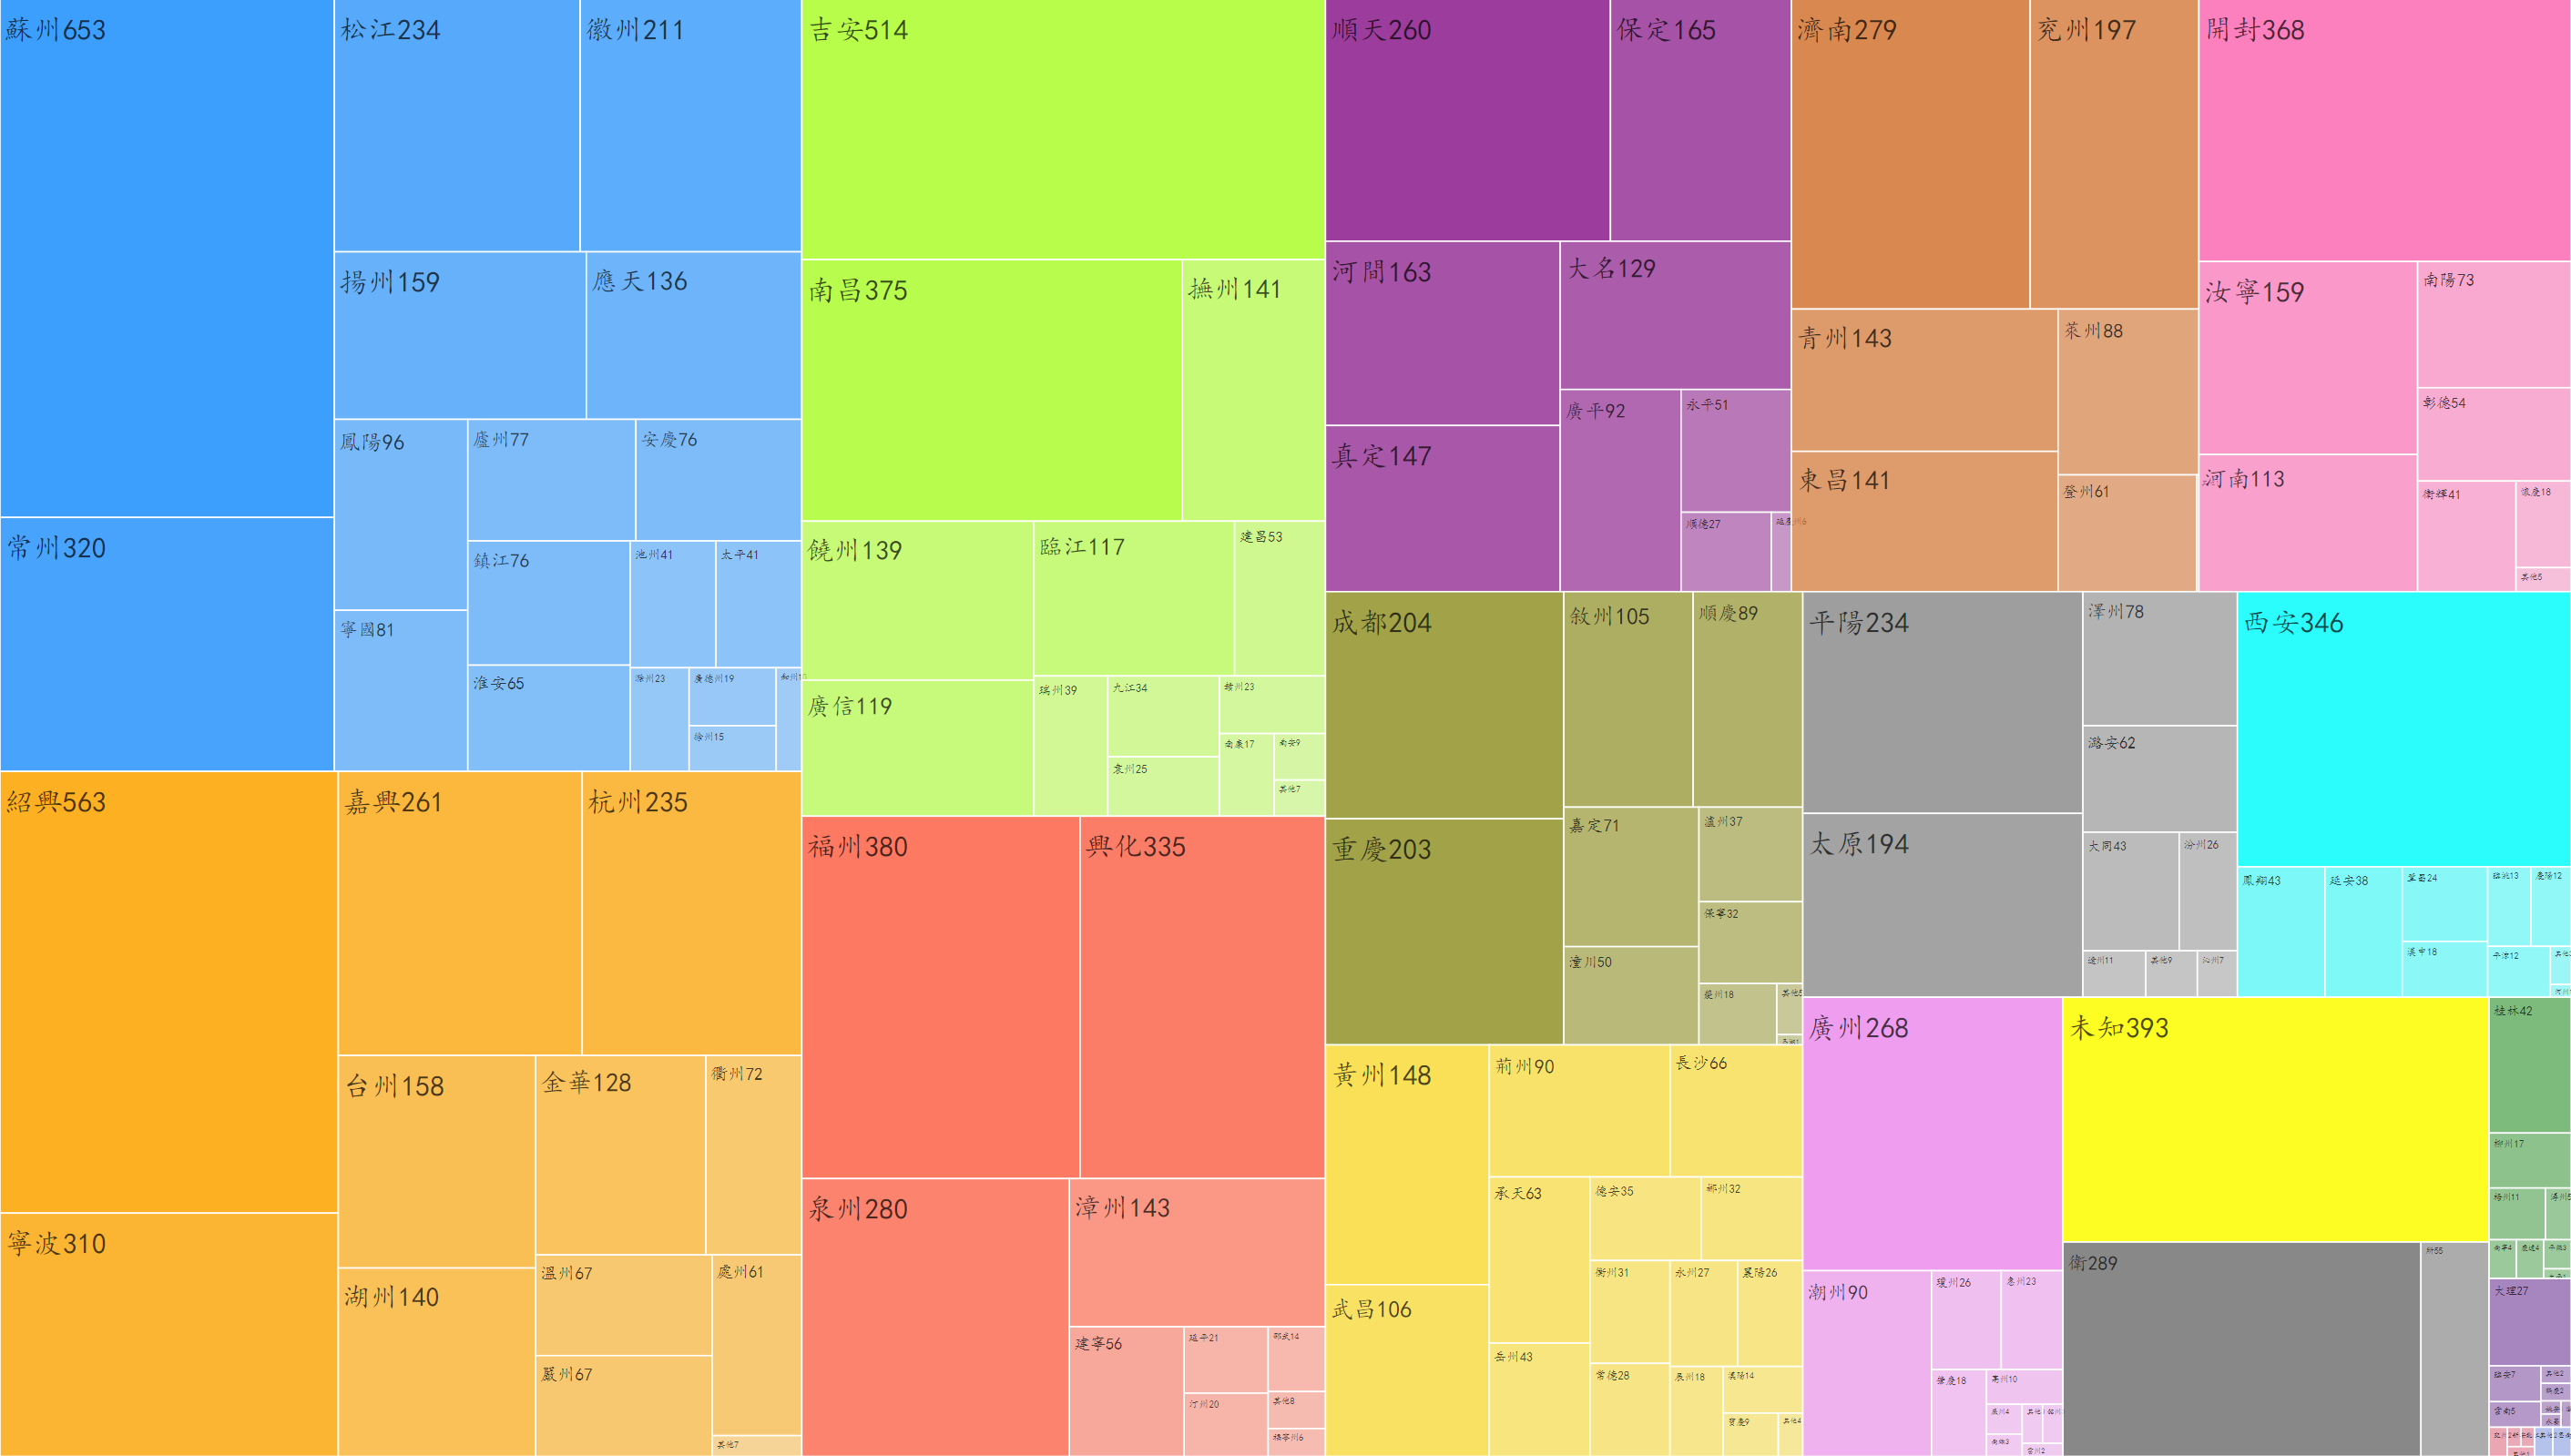
\includegraphics[width=10cm]{./figures/fu_squarified_treemap.png}
		\caption{Squarified Treemap of Fu-level}
	\end{figure}
	\begin{figure}[H]
		\centering
		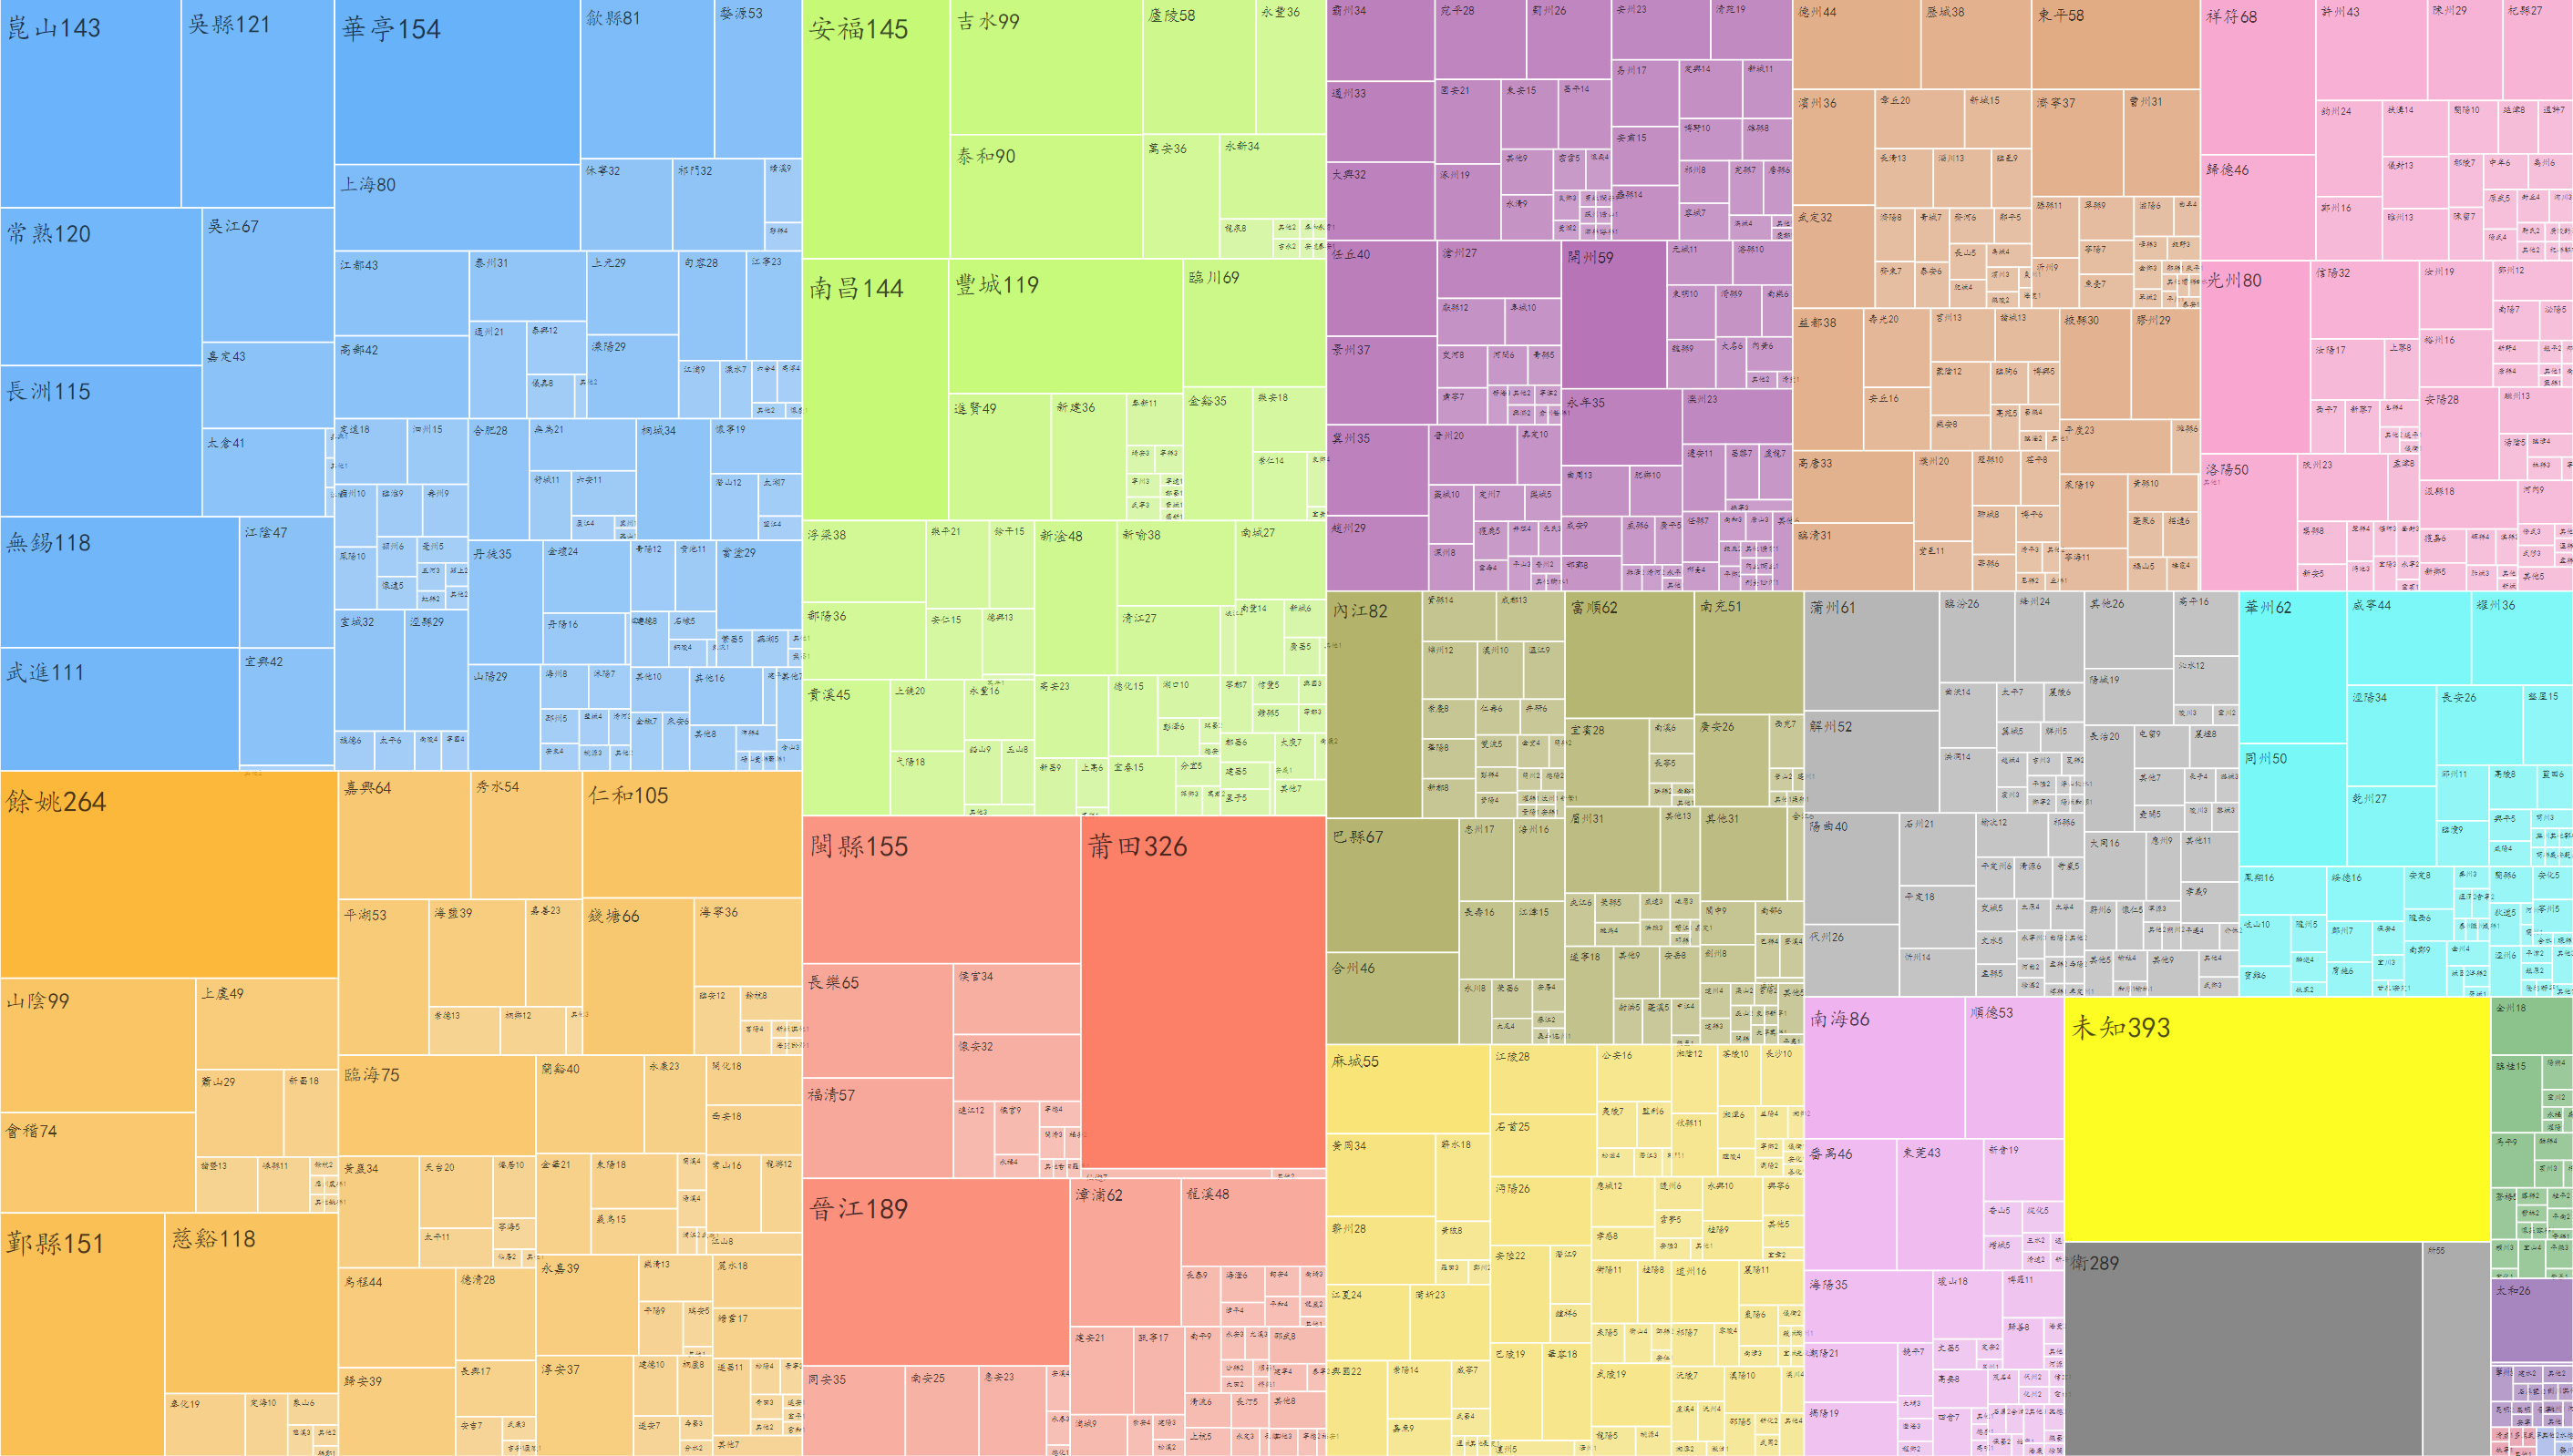
\includegraphics[width=10cm]{./figures/xian_squarified_treemap.png}
		\caption{Squarified Treemap of Xian-level}
	\end{figure}

	\begin{figure}[h]
		\begin{minipage}[h]{0.5\linewidth}
			\centering
			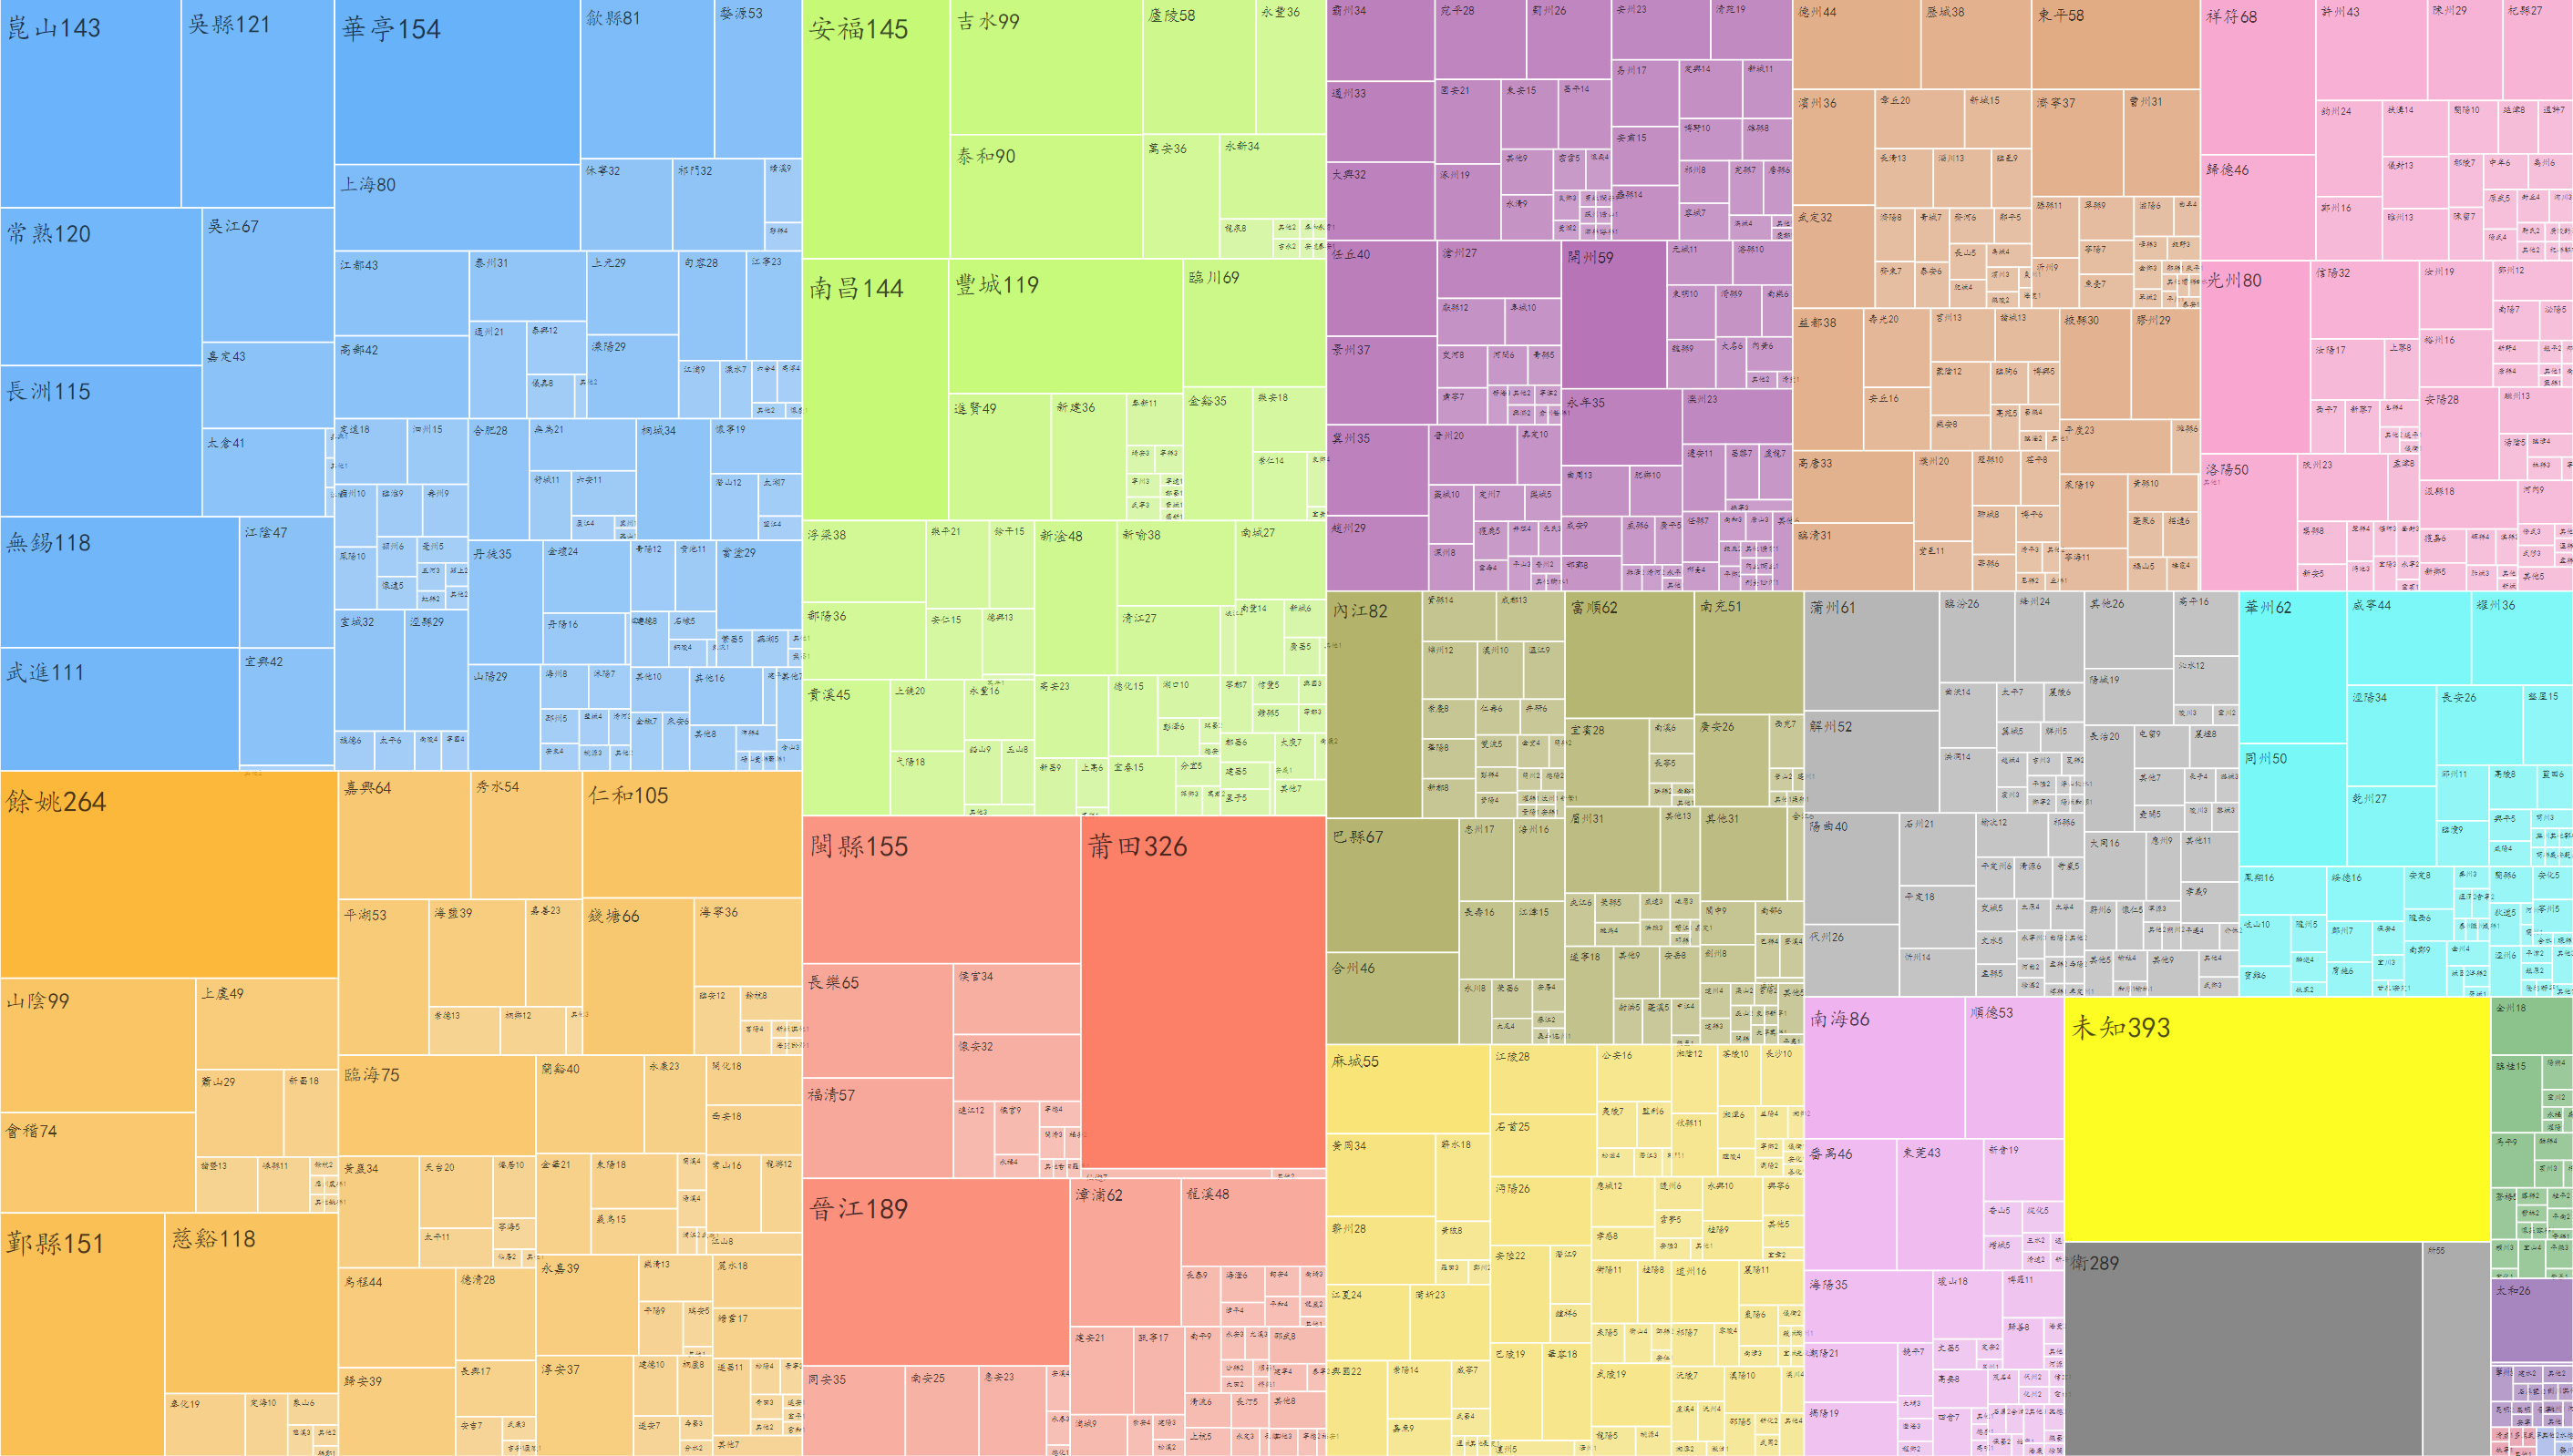
\includegraphics[width=0.9\textwidth]{./figures/xian_squarified_treemap.png}
			\caption{Squarified Treemap}
		\end{minipage}
		\begin{minipage}[h]{0.5\linewidth}
			\centering
			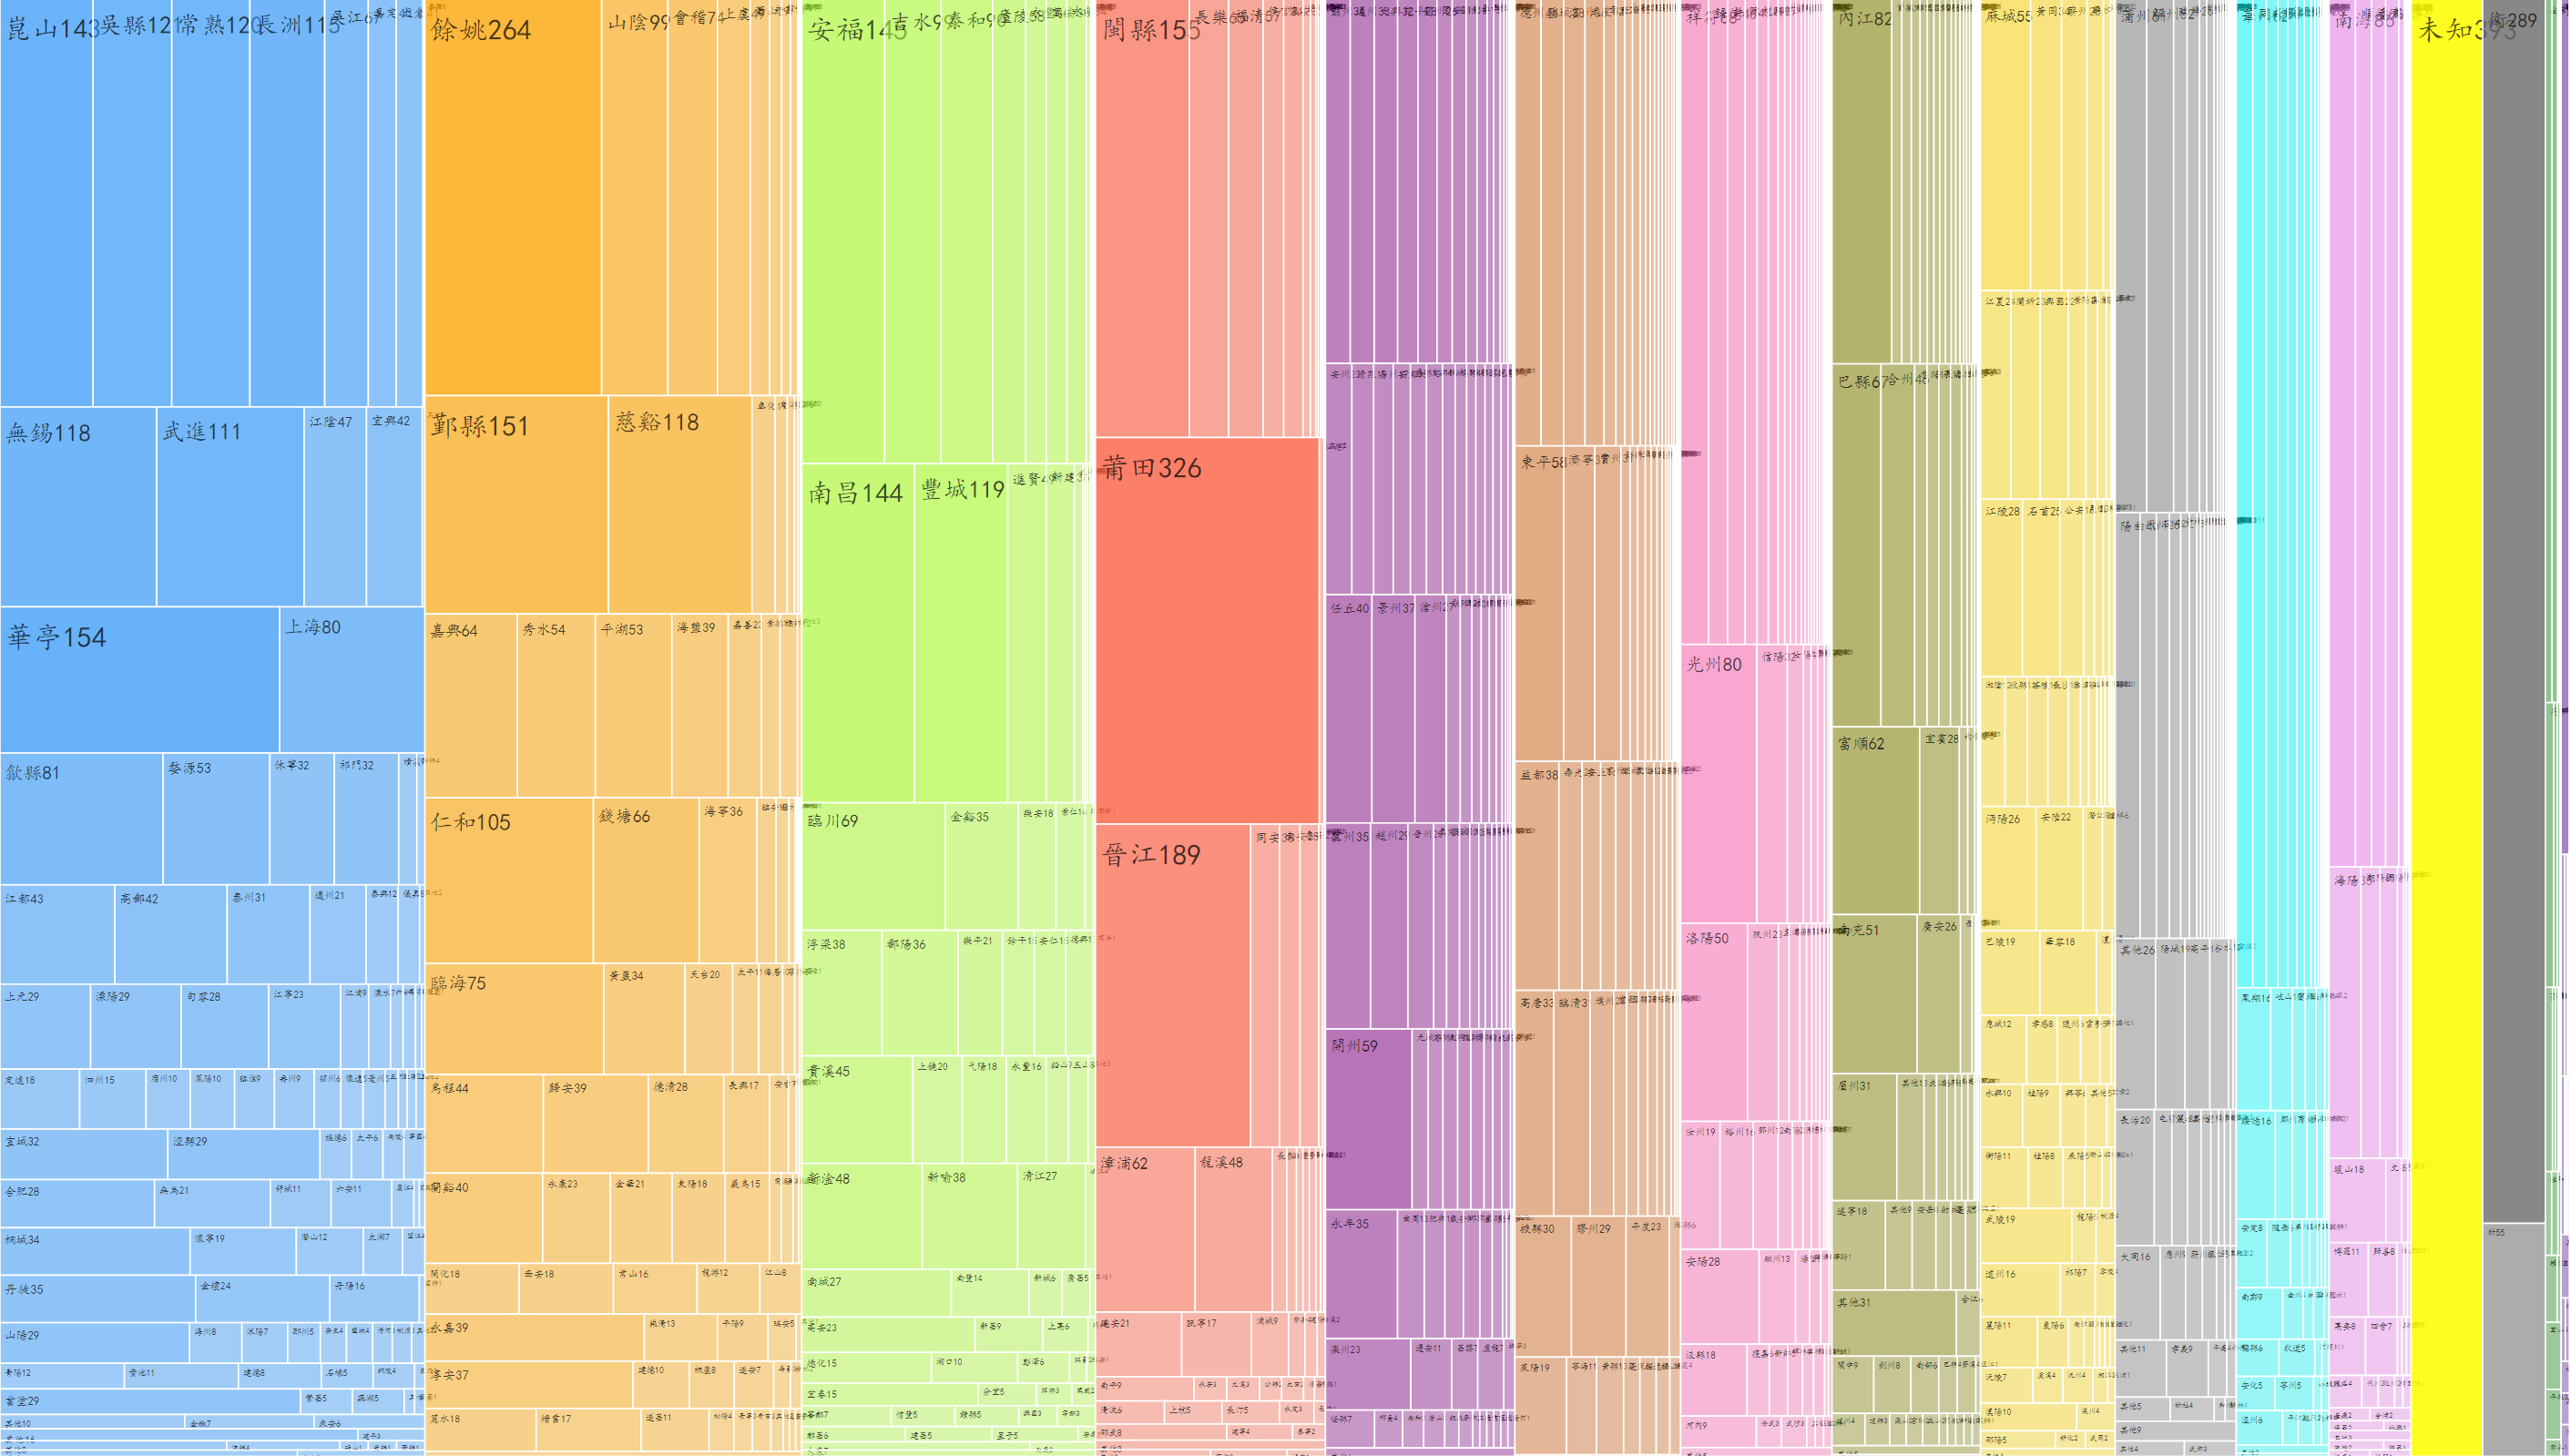
\includegraphics[width=0.9\textwidth]{./figures/xian_simple_treemap.png}
			\caption{Simple Treemap}
		\end{minipage}
	\end{figure}
	
	\subsection{总结与分析}
	从数据处理过程中发现,原始数据集存在诸多问题,如归类不清、错误记录等,但可利用一些手段最大限度地恢复数据中的真实信息,因此数据处理在可视化的任务中至关重要,往往也消耗了最多的时间(本次作业就是这样)。但好的数据处理也能够表现出巨大的功效,如在此次处理明进士籍贯的任务中,如果不加区分只是单纯简单地按照录入顺序清洗数据,划入未知类的数据可能达到两、三千条,但在精细地筛查后可将这一数字缩小至三、四百,减小了约一个数量级,能够为可视化提供更加准确的信息。
	
	\hspace*{\fill} \\
	
	从可视化结果中发现,历代考取进士最多的司级行政单位是南直隶(2333),最少的是贵州(4);最多的府级行政单位是苏州(653);最多的州县级行政单位则是莆田(326)。总体上各区域考取进士的人数与行政区划管辖面积及经济发展情况都正相关。南北直隶司下辖面积较大,考取进士人数相应多,而经济高度发展的江南地区(南直隶、浙江、江西)进士数量也均位居前列,较为偏远的交趾、贵州等地区教育程度则相对落后,考取进士零星(其中也有边远地区户籍管理不规范导致划分遗漏的原因)。大部分地区的进士考取都相对分散,只有福建等少数地区较为集中,这反映出当时中国的教育资源至少在司辖域内还是分配较为均衡的。同时,注意到两件有趣的事,其一是明代才子文武双全,在考中进士的14116人中便有344人可能出自军籍,与一个小型的司级行政区考取的人数相当;其二则是原始数据集中也出现了明代有记载的唯一一位外籍进士——高丽国金涛,他在洪武四年考中辛亥科三甲第五名进士,被授任县丞,而后本人以不通汉语为理由,请求回国,可谓是相当有意思了。
	
	\hspace*{\fill} \\
	
	从算法设计及最终实现过程中发现,Squarified Treemap算法绘制出的等方树图与简单树图相比小矩形的长宽比更趋向1,而正方形更易于观察与点击,故等方树图的可视化效果显然更优。而算法绘制出的等方树图的美观程度与小矩形面积及原始矩形的给定长宽关系紧密,绘制时应当保证小矩形面积之和等于原始矩形的面积(不相等时可将小矩形面积按比例扩大),否则将会留下大块空白区域,同时原始矩形的长宽比也至关重要,过大的长宽比同样会留下大片空白,而长宽趋向相等时很难与显示器尺寸适配,只有一个较小范围内的值可以适配当前数据,在绘制时需要反复调整。
	
\end{document}

%%%%%%%%%%%%%%%%%%%%%%%%%%%%Library%%%%%%%%%%%%%%%%%%%%%%%%%%%%%%%%%%%%%%%

% 1. 脚注用法
LaTeX\footnote{Latex is Latex} is a good software

%2. 强调
\emph{center of percussion} %[Brody 1986], %\lipsum[5]

%3. 随便生成一段话
\usepackage{lipsum}
\lipsum[4]

%4. 列条目
\begin{itemize}
	\item the angular velocity of the bat,
	\item the velocity of the ball, and
	\item the position of impact along the bat.
\end{itemize}

%5. 表格
\begin{table}[h]
	\centering  
	\begin{tabular}{c|cc}
		\hline
		年份 & \multicolumn{2}{c}{指标}\\
		\hline
		2017 & 0.9997 & 0.0555 \\
		2018 & 0.9994 & 0      \\
		2019 & 0.9993 & 0      \\
		\hline
	\end{tabular}
	\caption{NAME}\label{SIGN}
\end{table}

\begin{center}
	\begin{tabular}{c|cclcrcc}
		\hline
		Year & theta & $S_1^-$ & $S_2^-$ & $S_3^-$ & $S_4^+$ & $S_5^+$ & $S_6^+$ \\%表格标题
		\hline
		2016 & 1      & 0      & 0 & 0.0001 & 0      & 0      & 0 \\
		2017 & 0.9997 & 0.0555 & 0 & 0.2889 & 0.1844 & 0.463  & 0 \\
		2018 & 0.9994 & 0      & 0 & 0.0012 & 0.3269 & 0.7154 & 0 \\
		2019 & 0.9993 & 0      & 0 & 0      & 0.4325 & 1.0473 & 0 \\
		2020 & 0.9991 & 0      & 0 & 0      & 0.5046 & 1.2022 & 0 \\
		2021 & 0.999  & 0      & 0 & 0      & 0.5466 & 1.2827 & 0 \\
		2022 & 0.9989 & 0.0017 & 0 & 0.3159 & 0.562  & 1.2995 & 0 \\
		2023 & 0.9989 & 0      & 0 & 0.0109 & 0.5533 & 1.2616 & 0 \\
		2024 & 0.9989 & 0      & 0 & 0      & 0.5232 & 1.1769 & 0 \\
		2025 & 0.9989 & 0      & 0 & 0.1009 & 0.4738 & 1.0521 & 0 \\
		2026 & 0.9991 & 0      & 0 & 0      & 0.4071 & 0.8929 & 0 \\
		2027 & 0.9992 & 0.0004 & 0 & 0.1195 & 0.3248 & 0.7042 & 0 \\
		2028 & 0.9994 & 0.0164 & 0 & 0.046  & 0.2287 & 0.4902 & 0 \\
		2029 & 0.9997 & 0      & 0 & 0.0609 & 0.12   & 0.2545 & 0 \\
		2030 & 1      & 0      & 0 & 0      & 0      & 0      & 0 \\
		\hline
	\end{tabular}
\end{center}

%6. 数学公式
\begin{equation}
	a^2 = a * a\label{aa}
\end{equation}

\[
\begin{pmatrix}{*{20}c}
	{a_{11} } & {a_{12} } & {a_{13} }  \\
	{a_{21} } & {a_{22} } & {a_{23} }  \\
	{a_{31} } & {a_{32} } & {a_{33} }  \\
\end{pmatrix}
= \frac{{Opposite}}{{Hypotenuse}}\cos ^{ - 1} \theta \arcsin \theta
\]

\[
p_{j}=\begin{cases} 0,&\text{if $j$ is odd}\\
	r!\,(-1)^{j/2},&\text{if $j$ is even}
\end{cases}
\]


\[
\arcsin \theta  =
\mathop{{\int\!\!\!\!\!\int\!\!\!\!\!\int}\mkern-31.2mu
	\bigodot}\limits_\varphi
{\mathop {\lim }\limits_{x \to \infty } \frac{{n!}}{{r!\left( {n - r}
			\right)!}}} \eqno (1)
\]

%7. 双图并行
\begin{figure}[h]
	% 一个2*2图片的排列
	\begin{minipage}[h]{0.5\linewidth}
		\centering
		\includegraphics[width=0.8\textwidth]{./figures/0.jpg}
		\caption{Figure example 2}
	\end{minipage}
	\begin{minipage}[h]{0.5\linewidth}
		\centering
		\includegraphics[width=0.8\textwidth]{./figures/0.jpg}
		\caption{Figure example 3}
	\end{minipage}
\end{figure}

%8. 单张图片部分
\begin{figure}[h]
	%\small
	\centering
	\includegraphics[width=12cm]{./figures/mcmthesis-aaa.eps}
	\caption{Figure example 1} \label{fig:aa}
\end{figure}

%%%%%%%%%%%%%%%%%%%%%%%%%%%%%%%%%%%%%%%%%%%%%%%%%%%%%%%%%%%%%%%%%%%%%%%%%%%%%
\begin{minipage}{0.5\linewidth}
	\begin{tabular}{|c|c|c|}
		\hline
		\multicolumn{2}{|c|}{\multirow{2}{*}{合并}}&测试\\
		\cline{3-3}
		\multicolumn{2}{|c|}{}& 0.9997  \\
		\hline
		2019 & 0.9993 & 0 \\
		\hline
	\end{tabular}
\end{minipage}

\begin{minipage}{0.5\linewidth}
	\begin{tabular}{c|ccc}
		\hline
		年份 & \multicolumn{3}{c}{指标}\\
		\hline
		\multirow{3}{*}{合并}&2017 & 0.9997 & 0.0555 \\
		&2018 & 0.9994 & 0      \\
		&2019 & 0.9993 & 0      \\
		\hline
	\end{tabular}
\end{minipage}

\begin{table}[h]
	\centering	
	\begin{Large}
		\begin{tabular}{p{4cm} p{8cm} < {\centering}}
			\hline
			院\qquad 系: & 信息工程学院 \\
			\hline
			团队名称: & PlantBook Team \\
			\hline
			分\qquad 组: & 第0组1号 \\
			\hline
			日\qquad 期: & 2017年10月28日 \\
			\hline
			指导教师: & 吱吱吱\\
			\hline
		\end{tabular}
	\end{Large}
\end{table}

\ctexset{
	section={
		format+=\heiti \raggedright,
		name={,、},
		number=\chinese{section},
		beforeskip=1.0ex plus 0.2ex minus .2ex,
		afterskip=1.0ex plus 0.2ex minus .2ex,
		aftername=\hspace{0pt}
	},
}

\begin{table}[h]
	\centering
	\begin{Large}
		\begin{tabular}{p{3cm} p{7cm}<{\centering}}
			院  \qquad  系: & 信息工程学院           \\ \cline{2-2}
		\end{tabular}
	\end{Large}		
\end{table}
\thispagestyle{empty}
\newpage
\thispagestyle{empty}
\tableofcontents
\thispagestyle{empty}
\newpage
\setcounter{page}{1}

% 9. 代码
\usepackage{listings}
\usepackage{xcolor}
\lstset{
	numbers=left, 
	numberstyle= \tiny, 
	keywordstyle= \color{ blue!70},
	commentstyle= \color{red!50!green!50!blue!50}, 
	frame=shadowbox, % 阴影效果
	rulesepcolor= \color{ red!20!green!20!blue!20} ,
	escapeinside=``, % 英文分号中可写入中文
	xleftmargin=2em,xrightmargin=2em, aboveskip=1em,
	basicstyle=\footnotesize,
	framexleftmargin=2em
}
